\documentclass[14pt,aspectratio=1610]{beamer}

\usepackage[brazil]{babel}
\usepackage[utf8]{inputenc}
%\UseRawInputEncoding
\usepackage[T1]{fontenc}
%\usepackage{Sweave}
\usepackage{animate}
\usepackage{amsbsy}
\usepackage{amsfonts}
\usepackage{amsmath}
\usepackage{amssymb}
\usepackage{amsthm}
\usepackage[toc,page,title,titletoc]{appendix}
%\usepackage[fixlanguage]{babelbib}
%\usepackage[pdftex]{color}
\usepackage{dsfont}
\usepackage{esvect}
\usepackage[labelfont=bf]{caption}
\usepackage{subcaption}
\usepackage{float}
\usepackage[Glenn]{fncychap}%Sonny %Conny %Lenny %Glenn %Renje %Bjarne %Bjornstrup
%\usepackage{geometry, calc, color, setspace}%
%\geometry{a4paper, headsep=1.0cm, footskip=1cm, lmargin=3cm, rmargin=2cm, tmargin=3cm, bmargin=2cm}
\usepackage{graphicx}
\usepackage{indentfirst}%Para indentar os parágrafos automáticamente
\usepackage{lipsum}
\usepackage{longtable}
\usepackage{mathtools}
\usepackage{listings}%Inserir codigo do R no latex
%\usepackage{slashbox}
\usepackage{multirow}
\usepackage{multicol}
\usepackage{csquotes}
\usepackage[maxcitenames=2,terseinits=true,natbib=true, style=authoryear, maxbibnames=99]{biblatex}
\addbibresource{../Referencias/Referencias.bib}
\usepackage[figuresright]{rotating}
\usepackage{spalign}
%\usepackage{pgfpages}
\usepackage{pgfplots}
\pgfplotsset{compat=1.18}
\usepackage{tikz}
\usepackage{color, colortbl}
\usepackage{ragged2e}%para justificar o texto dentro de algum ambiente
\definecolor{Gray}{gray}{0.9}
\definecolor{LightCyan}{rgb}{0.88,1,1}
\definecolor{Lightblue}{RGB}{50, 149, 168}
%\usepackage{grffile}

\usepackage[all]{xy}



%\usetheme{Madrid}
%\usecolortheme[RGB={193,0,0}]{structure}
\usetheme{metropolis}
\definecolor{mycolor}{RGB}{34, 45, 50}
\setbeamercolor{structure}{fg=mycolor}
\usepackage{mathpazo} % Fonte elegante para matemática
\usepackage{helvet} % Fonte sans-serif para texto
\renewcommand{\familydefault}{\sfdefault} % Definir fonte padrão como sans-serif

%\setbeamertemplate{footline}[frame number]
%\setbeamertemplate{footline}[text line]{%
	%  \parbox{\linewidth}{\vspace*{-8pt}\hfill\date{}\hfill\insertshortauthor\hfill\insertpagenumber}}
\beamertemplatenavigationsymbolsempty
\renewcommand{\vec}[1]{\mbox{\boldmath$#1$}}
\newtheorem{Teorema}{Teorema}
\newtheorem{Proposicao}{Proposição}
\newtheorem{Definicao}{Definição}
\newtheorem{Corolario}{Corolário}
\newtheorem{Demonstracao}{Demonstração}
\newcommand{\bx}{\ensuremath{\bar{x}}}
\newcommand{\Ho}{\ensuremath{H_{0}}}
\newcommand{\Hi}{\ensuremath{H_{1}}}
\everymath{\displaystyle}

\apptocmd{\frame}{}{\justifying}{} % Allow optional arguments after frame.

\title{Estatística I}
\author{Prof. Fernando de Souza Bastos \texorpdfstring{\\ fernando.bastos@ufv.br}{}}
\institute{Departamento de Estatística \texorpdfstring{\\ Universidade Federal de Viçosa}{}\texorpdfstring{\\ Campus UFV - Viçosa}{}}
\date{}
\newcommand\mytext{Aula 19}
\newcommand\mytextt{Fernando de Souza Bastos}
\newcommand\mytexttt{\url{https://ufvest.github.io/}}

\makeatletter
\setbeamertemplate{footline}
{
	\leavevmode%
	\hbox{%
		\begin{beamercolorbox}[wd=.3\paperwidth,ht=2.25ex,dp=1ex,center]{author in head/foot}%
			\usebeamerfont{author in head/foot}\mytext
		\end{beamercolorbox}%
		\begin{beamercolorbox}[wd=.3\paperwidth,ht=2.25ex,dp=1ex,center]{title in head/foot}%
			\usebeamerfont{title in head/foot}\mytextt
		\end{beamercolorbox}%
		\begin{beamercolorbox}[wd=.35\paperwidth,ht=2.25ex,dp=1ex,right]{site in head/foot}%
			\usebeamerfont{site in head/foot}\mytexttt\hspace*{2em}
			\insertframenumber{} / \inserttotalframenumber\hspace*{2ex} 
	\end{beamercolorbox}}%
	\vskip0pt%
}
\makeatother

\providecommand{\arcsin}{} \renewcommand{\arcsin}{\hspace{2pt}\textrm{arcsen}}
\providecommand{\sin}{} \renewcommand{\sin}{\hspace{2pt}\textrm{sen}}
%\newtheorem{Teorema}{Teorema}
%\newtheorem{Proposicao}{Proposição}
%\newtheorem{Definicao}{Definição}
%\newtheorem{Corolario}{Corolário}
%\newtheorem{Demonstracao}{Demonstração}

\titlegraphic{\hspace*{8cm}\href{https://fsbmat-ufv.github.io/}{
\includegraphics[width=2cm]{figs/mylogo.png}}
}


\usepackage{hyperref,bookmark}
\hypersetup{
	colorlinks=true,
	linkcolor=blue,
	citecolor=red,
	filecolor=blue,
	urlcolor=blue,
}

% Layout da pagina
\hypersetup{pdfpagelayout=SinglePage}
\begin{document}
	%\input{Aula21-concordance}
	
	\frame{\titlepage}
	
	\begin{frame}{}
		\frametitle{\bf Sumário}
		\tableofcontents
	\end{frame}
	
\section{Introdução}

\begin{frame}{Por que não confiar só na média?}
	
	\begin{block}{}
		\justifying
		
		Imagine que você está com muita fome e abre o aplicativo de delivery. A informação aparece assim:
		
		\begin{center}
			\textbf{"O tempo médio de entrega é de 30 minutos."}
		\end{center}
		
		Você pensa:
		
		\textit{"Perfeito! Em meia horinha eu tô comendo!"}
		
	\end{block}
	
\end{frame}

\begin{frame}{Por que não confiar só na média?}
	
	\begin{block}{}
		\justifying
		
		Mas... será que é tão simples assim?
		
		Pense nos dados que o aplicativo usa para calcular essa média:
		
		\begin{itemize}
			\item Algumas entregas foram muito rápidas (15, 20 minutos).
			\item Outras demoraram bastante (60, 70, até 90 minutos).
		\end{itemize}
		
		A \textbf{média} de 30 minutos parece bonita... mas esconde toda essa variabilidade!
		
	\end{block}
	
\end{frame}

\begin{frame}{A verdade por trás da média}
	\small
	\begin{block}{}
		\justifying
		
		Se o aplicativo dissesse:
		
		\begin{center}
			\textbf{"Com 95\% de confiança, seu pedido chegará entre 20 minutos e 1 hora e 10 minutos."}
		\end{center}
		
		Agora sim, você entende o jogo!
		
		Isso significa que:
		
		\begin{itemize}
			\item É possível que chegue rápido (20 min).
			\item Mas também existe uma chance real de demorar mais de uma hora.
		\end{itemize}
		
		\textbf{Percebe a diferença?}
		
		\begin{center}
			\textit{"A média é uma informação solitária. O intervalo de confiança é uma informação honesta."}
		\end{center}
		
	\end{block}
	
\end{frame}

\begin{frame}{}
	
	\begin{block}{}
		\justifying
		
		\begin{center}
			\textit{"A média é uma informação solitária. O intervalo de confiança é uma informação honesta."}
		\end{center}
		\pause
		\begin{center}
			\textit{Confiar só na média é como dirigir olhando apenas pelo retrovisor... Parece informação, mas não te mostra o que vem pela frente.}
		\end{center}
		
	\end{block}
\end{frame}	
	
	\begin{frame}{Dois tipos de estimativas}
		
		\begin{block}{Estimativa Pontual}
			\justifying
			É quando usamos um único número, calculado a partir da amostra, para estimar um parâmetro populacional.
			
			\vspace{0.2cm}
			\textbf{Exemplos:}
			\begin{itemize}
				\item Média amostral (\( \bar{x} \)) para estimar a média populacional (\( \mu \)).
				\item Proporção amostral (\( \hat{p} \)) para estimar a proporção populacional (\( p \)).
			\end{itemize}
			
			\textbf{Limitação:} Fornece apenas um valor. Não diz nada sobre a incerteza ou confiabilidade desse valor.
		\end{block}
		
	\end{frame}
	
	\begin{frame}{Dois tipos de estimativas}
			
		\begin{block}{Estimativa Intervalar (Intervalo de Confiança)}
			\justifying
			Em vez de fornecer um único número, fornece um \textbf{intervalo de valores plausíveis} para o parâmetro populacional.
			
			\vspace{0.2cm}
			\textbf{Exemplo:}
			\begin{center}
				\textit{"Com 95\% de confiança, a média populacional está entre 25 e 35."}
			\end{center}
			
			\textbf{Vantagem:} Expressa não só a estimativa, mas também a incerteza associada a ela.
		\end{block}
		
	\end{frame}
	
	\begin{frame}{Por que precisamos de um intervalo de confiança?}
		\small
		\vspace{-0.3cm}
		\begin{block}{}
			\justifying
			
			Todo estimador (como a média amostral) é uma \textbf{variável aleatória}.
				\vspace{-0.3cm}
			\begin{itemize}
				\item Se coletarmos outra amostra, vamos obter outro valor.
				\item A cada amostra possível, temos uma média diferente.
			\end{itemize}
				\vspace{-0.3cm}
			Por isso, o estimador possui uma \textbf{distribuição de probabilidade}, chamada de \textbf{distribuição amostral}.
			
			\textbf{E é exatamente a partir dessa distribuição que construímos o intervalo de confiança.}

			
			O intervalo de confiança nos permite afirmar algo do tipo:
			
			\begin{center}
				\textit{"Se eu repetir esse processo muitas vezes, 95\% dos intervalos conterão o verdadeiro valor do parâmetro."}
			\end{center}
			
		\end{block}
		
	\end{frame}
	

\begin{frame}{Visualizando a incerteza}
	\vspace{-0.3cm}
	\begin{block}{}
		\centering
		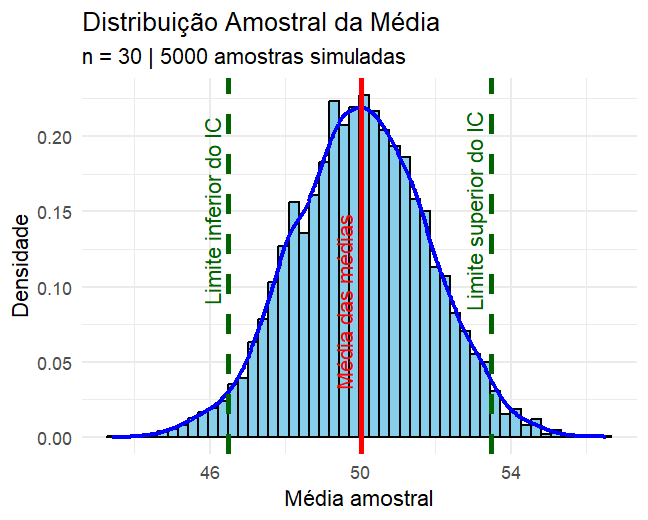
\includegraphics[width=0.7\linewidth]{figs/Intervalo.png}
	\end{block}
	
\end{frame}

	
\section{Intervalos de Confiança para a Média: $\sigma$ conhecido}

\begin{frame}{Suposições Necessárias}
	\begin{block}{}
		\justifying
		Para construirmos um intervalo de confiança para a média (com $\sigma$ conhecido), precisamos garantir:
		\begin{itemize}
			\item A amostra é uma \textbf{amostra aleatória simples (AAS)}.
			\item O desvio padrão da população ($\sigma$) é conhecido.
			\item E uma das seguintes condições:
			\begin{itemize}
				\item A população tem distribuição normal;
				\item ou o tamanho da amostra é suficientemente grande ($n > 30$).
			\end{itemize}
		\end{itemize}
	\end{block}
\end{frame}

\begin{frame}{Erro Amostral: Sempre Existe!}
	\small
	\begin{block}{}
		\justifying
		Ao coletar uma amostra, a média amostral ($\bar{X}$) dificilmente será exatamente igual à média populacional ($\mu$).
		
		\textbf{Essa diferença é chamada de erro amostral:}
		
		\[
		e = \bar{X} - \mu \quad \Leftrightarrow \quad \bar{X} = \mu + e
		\]
		
		Sabemos que a média amostral segue uma distribuição:
		
		\[
		\bar{X} \sim \text{N}\left(\mu, \frac{\sigma^2}{n}\right)
		\]
		
		Ou seja, as médias amostrais \textbf{variam} de amostra para amostra!
	\end{block}
\end{frame}

\begin{frame}{O que é a Margem de Erro?}
	\small
	\vspace{-0.3cm}
	\begin{block}{}
		\justifying
		Se padronizarmos a média amostral, obtemos:
		
		\[
		Z = \frac{\bar{X} - \mu}{\sigma / \sqrt{n}} \sim \text{N}(0,1)
		\]
		
		\textbf{Z responde:} Quantos desvios padrão minha média amostral está distante da média populacional.
		
		A \textbf{margem de erro} ($e$) representa o erro máximo aceitável, dentro de um grau de confiança ($\gamma$):
		
		\[
		e = z_{\gamma/2} \cdot \frac{\sigma}{\sqrt{n}}
		\]
		
		Onde $z_{\gamma/2}$ é o \textbf{valor crítico da normal padrão}.
	\end{block}
\end{frame}

\begin{frame}{Construindo o Intervalo de Confiança}
	\begin{block}{Raciocínio}
		\justifying
		Queremos capturar o valor de $\mu$ dentro de um intervalo simétrico ao redor da média amostral $\bar{x}$.
		\vspace{-0.3cm}
		\[
		P\left( -z_{\gamma/2} < Z < z_{\gamma/2} \right) = \gamma
		\]
			\vspace{-0.3cm}
		Substituindo $Z$ pela padronização da média:
		
		\[
		P\left( \bar{x} - z_{\gamma/2} \cdot \frac{\sigma}{\sqrt{n}} < \mu < \bar{x} + z_{\gamma/2} \cdot \frac{\sigma}{\sqrt{n}} \right) = \gamma
		\]
		
		\textbf{Pronto!} Este é o intervalo de confiança para $\mu$ com confiança $\gamma$.
	\end{block}
\end{frame}

\begin{frame}{Valor Crítico $z_{\gamma/2}$}
	\begin{block}{}
		\justifying
		O valor $z_{\gamma/2}$ é o ponto da distribuição normal padrão que deixa uma área de $\gamma/2$ em cada cauda.
		
		Por exemplo, para $\gamma = 0,95$:
		\begin{itemize}
			\item A área central é 95\%.
			\item Sobra 5\% para as caudas → 2,5\% em cada lado.
			\item Buscamos na tabela da normal padrão a área acumulada até 0,975.
			\item Resultado: $z_{0,025} = 1,96$.
		\end{itemize}
	\end{block}
	
	\centering
	%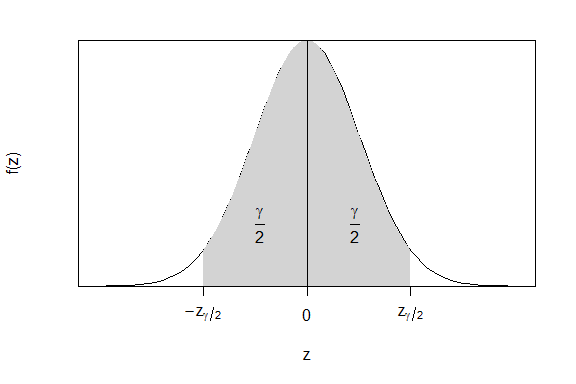
\includegraphics[width=0.75\linewidth]{figs/IC2.png}
	
	\small\textit{A área central corresponde ao nível de confiança $\gamma$.}
\end{frame}

\begin{frame}{Fórmula do Intervalo de Confiança}
	\begin{block}{}
		O intervalo de confiança para $\mu$, com nível de confiança $\gamma$, é dado por:
		
		\[
		\left[
		\bar{X} - z_{\gamma/2} \cdot \frac{\sigma}{\sqrt{n}} \; ; \;
		\bar{X} + z_{\gamma/2} \cdot \frac{\sigma}{\sqrt{n}}
		\right]
		\]
		
		\textbf{Interpretação:} Uma faixa de valores plausíveis para a média populacional, considerando a variabilidade natural das amostras.
	\end{block}
\end{frame}

\begin{frame}{Passos para construir o Intervalo de Confiança}
	\begin{enumerate}
		\item Verificar as suposições:
		\begin{itemize}
			\item AAS
			\item $\sigma$ conhecido
			\item População normal ou $n > 30$
		\end{itemize}
		\item Escolher o nível de confiança $\gamma$ e determinar $z_{\gamma/2}$.
		\item Calcular a margem de erro:
		\[
		e = z_{\gamma/2} \cdot \frac{\sigma}{\sqrt{n}}
		\]
		\item Construir o intervalo:
		\[
		\bar{X} \pm e
		\]
	\end{enumerate}
\end{frame}

\begin{frame}{Interpretação do Intervalo de Confiança}
	\begin{block}{Atenção: O que significa $\gamma$?}
		\justifying
		- O \textbf{parâmetro} ($\mu$) é fixo.  
		- O que varia é o \textbf{intervalo}, porque ele depende da amostra.  
		
		Se construirmos 100 intervalos de confiança de 95\%, usando 100 amostras diferentes, \textbf{esperamos que 95 deles contenham $\mu$}, e 5 não contenham.
		
		\textbf{Importante:} \textit{Não dizemos que "a chance de $\mu$ estar no intervalo é 95\%". $\mu$ não é aleatório. O que é aleatório é o intervalo.}
	\end{block}
\end{frame}

	
	\begin{frame}{}
		\begin{block}{}
			\justifying
			\begin{figure}
				\centering
				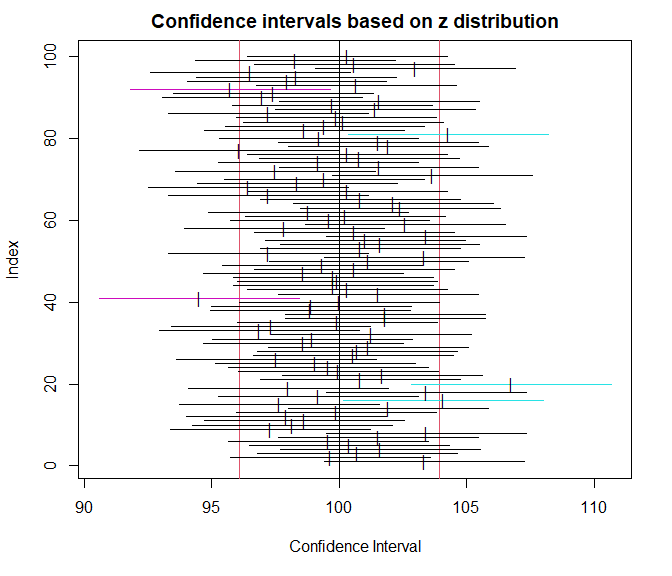
\includegraphics[scale=0.6]{figs/IC3.png}
			\end{figure}
		\end{block}
	\end{frame}
	
	\begin{frame}{Exemplo}
		\begin{block}{}
			\justifying
			Uma empresa de computadores deseja estimar o tempo médio de horas semanais que as pessoas utilizam o computador. Uma amostra aleatória de 25 pessoas apresentou um tempo médio de uso de 22,4 horas. Com base em estudos anteriores, a empresa assume que $\sigma = 5,2$ horas, e que os tempos são normalmente distribuídos. Construa um intervalo de confiança para a média $\mu$ com coeficiente de confiança de 95%.   
		\end{block}
		\pause 
		\begin{block}{}
			%\begin{verbatim}
			%xbar <- 22.4
			%n <- 25
			%sigma <- 5.2
			%zcrit <- qnorm(.975)
			%erro <- zcrit * sigma/sqrt(n)
			%c(xbar - erro, xbar + erro)
			$(20.36164\leq \mu\leq24.43836)$
			%\end{verbatim}   
		\end{block}
	\end{frame}
	
	\section{Intervalos de confiança para a média: $\sigma$ desconhecido}
	\begin{frame}{Intervalos de confiança para a média: $\sigma$ desconhecido}
		\begin{block}{Estimativa da variância amostral}
			\justifying
			Na maioria das situações práticas, não sabemos o verdadeiro valor do desvio padrão populacional $\sigma$. Se o desvio padrão é desconhecido, ele precisa ser estimado. Sendo $(X_1, \ldots, X_n)$ VAs onde $X \sim \text{N}(\mu, \sigma^2)$, vimos que o ``melhor'' estimador para $\sigma^2$ é a variância amostral
			$$
			S^2 = \frac{1}{n-1} (\sum_{i=1}^{n} X_i^2 - n\bar{X}^2)
			$$   
			que é não viciada e consistente para $\sigma^2$.   
		\end{block}
	\end{frame}
	
	\begin{frame}{A distribuição $t$ de Student}
		\begin{block}{}
			\justifying
			Definindo a variável padronizada
			$$
			T = \frac{\bar{X} - \mu}{\sqrt{S^2/n}} = \frac{\bar{X} - \mu}{S/\sqrt{n}}
			$$   
			o denominador $S^2$ fará com que a função densidade de $T$ seja diferente da Normal. Essa nova densidade é denominada \textbf{$t$ de Student}, e seu parâmetro é
			denominado \textbf{graus de liberdade}, que nesse caso é $n-1$. Assim:
			$$
			T = \frac{\bar{X} - \mu}{S/\sqrt{n}} \, \sim \, t(n-1)
			$$   
		\end{block}
	\end{frame}
	
	\begin{frame}{}
		\begin{block}{Valores Críticos de $t$}
			\justifying
			Com a definição do \textbf{nível de confiança} e sabendo o tamanho da amostra $n$, sabemos então o valor de $\gamma$ e dos gl, e devemos encontrar o \textbf{valor crítico} de $t_{\gamma/2}$. Usando como exemplo $\gamma = 0,95$ e uma amostra de $n=7$
			
			\begin{itemize}
				\item Temos que $n=7 \Rightarrow gl = n-1 = 6$
				
				\item Na tabela da distribuição $t$ de Student procure a linha correspondente aos gl, e  coluna correspondente ao valor de $1 - \gamma = 1 - 0,95 = 0,05 = 5\%$
				
				\item O valor de $t_{\gamma/2}$ será determinado pelos valores correspondentes \textbf{no corpo da tabela}. Nesse caso, $t_{\gamma/2} = 2,447$ é o valor crítico procurado.
			\end{itemize}   
		\end{block}
	\end{frame}
	
	\begin{frame}{}
		\begin{block}{}
			\justifying
			\begin{figure}
				\centering
				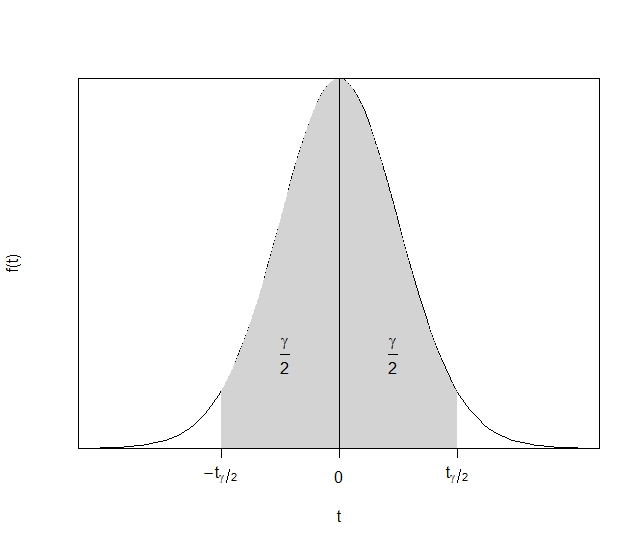
\includegraphics[scale=0.6]{figs/ICtStudent.jpeg}
			\end{figure}  
		\end{block}
	\end{frame}
	
	\begin{frame}{Intervalo de confiança}
		\begin{block}{}
			\justifying
			Com estas definições, podemos construir um \textbf{intervalo de confiança} para $\mu$, com \textbf{coeficiente de confiança} $\gamma$, e
			$\sigma$ desconhecido:
			$$
			\text{IC}(\mu, \gamma) = \left[ \bar{X} - t_{\gamma/2} \cdot
			\left(\frac{S}{\sqrt{n}}\right) ; \bar{X} + t_{\gamma/2} \cdot
			\left(\frac{S}{\sqrt{n}}\right)  \right]
			$$   
			
		\end{block}
	\end{frame}
	
	\begin{frame}{Procedimentos para a construção de intervalos de confiança}
		\begin{block}{}
			\justifying
			\begin{enumerate}
				\item Verifique se as suposições necessárias estão satisfeitas
				\begin{itemize}
					\item Temos uma AAS
					\item Temos uma estimativa de $s$
					\item A população tem distribuição normal ou $n>30$
				\end{itemize}
				
				\item Determine o nível de confiança $\gamma$, e encontre o valor crítico $t_{\gamma/2}$
				\item Calcule a margem de erro $e = t_{\gamma/2} \cdot (s/\sqrt{n})$
				\item Calcule $\text{IC}(\mu, \gamma)$
			\end{enumerate}   
		\end{block}
	\end{frame}
	
	\begin{frame}{}
		\begin{block}{Exemplo}
			\justifying
			Em um teste da eficácia do alho na dieta para a redução do colesterol, 51 pessoas foram avaliadas e seus níveis de colesterol foram medidos antes e depois do tratamento. As \textbf{mudanças} nos níveis de colesterol apresentaram média de 0,4 e desvio-padrão de
			21. 
			\begin{description}
				\item[a)~]Para um nível de confiança de 95\%, calcule o intervalo para a verdadeira média das mudanças no nível de colesterol;
				\item[b)~]O que o intervalo de confiança sugere sobre a eficácia do uso do alho na dieta para a redução do colesterol?
				\item[c)~]Resolva o mesmo exemplo supondo que o $\sigma = s$ é conhecido (ou seja, usando a distribuição $Z$). Compare os dois métodos.
			\end{description}
		\end{block}
	\end{frame}
	
	\section{Intervalo de Confiança para Proporção}
	\begin{frame}{Intervalo de Confiança para Proporção}
		\vspace{-0.3cm}
		\begin{block}{}
			\justifying
			A proporção amostral
			$$
			\hat{p} = \frac{x}{n} = \frac{\text{número de sucessos}}{\text{total de
					tentativas}}
			$$   
			é a ``melhor estimativa'' para a proporção populacional $p.$ Através do estudo da distribuição amostral da proporção, chegamos aos seguintes resultados:
			
			\begin{itemize}
				\item A proporção amostral $\hat{p}$ \textbf{tende} para o valor da proporção populacional $p$
				\item A distribuição das proporções amostrais tende a ser uma \textbf{distribuição normal}
				\item $\text{E}(\hat{p}) = \mu_{\hat{p}} = p$
				\item $\text{Var}(\hat{p}) = \sigma^{2}_{\hat{p}} = \frac{p(1-p)}{n}$
			\end{itemize}
		\end{block}
	\end{frame}
	
	\begin{frame}{Distribuição amostral da proporção $\hat{p}$}
		\begin{block}{}
			\justifying
			Assim, sabemos que
			$$
			\hat{p} \sim \text{N} \left( p, \frac{p(1-p)}{n} \right)
			$$   
			É possível mostrar que a quantidade
			$$
			Z = \frac{\hat{p} - p}{\sqrt{\frac{p(1-p)}{n}}} \, \sim \, \text{N}(0,1)
			$$   
		\end{block}
	\end{frame}
	
	\begin{frame}{}
		\begin{block}{Intervalo de Confiança}
			\justifying
			Logo, podemos construir um \textbf{intervalo de confiança} para $p$, com \textbf{coeficiente de confiança} $\gamma$
			$$
			\text{IC}(p, \gamma) = \left[ \hat{p} - z_{\gamma/2} \cdot
			\sqrt{\frac{p(1-p)}{n}} ;
			\hat{p} + z_{\gamma/2} \cdot
			\sqrt{\frac{p(1-p)}{n}}
			\right]
			$$
		\end{block}
	\end{frame}
	
	\begin{frame}{Procedimentos para a construção de intervalos de confiança}
		\begin{block}{}
			\justifying
			\begin{enumerate}
				\item Verifique se as suposições necessárias estão satisfeitas
				\begin{itemize}
					\item Temos uma AAS
					\item As condições para a distribuição binomial são satisfeitas:
					\begin{itemize}
						\item as tentativas são independentes;
						\item há duas categorias de resultado (``sucesso'', ``fracasso'');
						\item a probabilidade de sucesso $p$ permanece constante;
					\end{itemize}
					\item A distribuição normal pode ser usada como aproximação para a    distribuição binomial, ou seja, $np \geq 5$ e $np(1-p) \geq 5$
				\end{itemize}
				
				\item Determine o nível de confiança $\gamma$, e encontre o valor crítico $z_{\gamma/2}$
				\item Calcule a margem de erro $e = z_{\gamma/2} \cdot \sqrt{\frac{p(1-p)}{n}}$
				\item Calcule $\text{IC}(\mu, \gamma)$
			\end{enumerate}   
		\end{block}
	\end{frame}
	
	\begin{frame}{}
		\begin{block}{Exemplo}
			\justifying
			Em uma pesquisa realizada por um instituto de pesquisa Norte-Americano, 1500 adultos foram selecionados aleatoriamente para responder à pergunta se acreditam ou não no aquecimento global. 1050 entrevistados responderam que sim. Com isso:
			
			\begin{description}
				\item[a)~]Para um nível de confiança de 95\%, calcule o intervalo de confiança para a verdadeira proporção de pessoas que acreditam no aquecimento global, utilizando:
				$(i)\ p = \hat{p} \text{ e } (ii)\ p = 0,5$ e compare os resultados.
				\item[b)~]Com base nesses resultados, podemos concluir que a maioria dos adultos acredita no aquecimento global?
			\end{description}   
		\end{block}
	\end{frame}
	
	\section{Determinação do tamanho amostral ($\sigma$ conhecido)}
	\begin{frame}{Determinação do tamanho amostral}
		\begin{block}{}
			\justifying
			Nosso objetivo é coletar dados para estimar a \textbf{média populacional} $\mu$. A questão é:
			\begin{center}
				\textbf{Quantos elementos (itens, objetos, pessoas, ...) devemos amostrar?}   
			\end{center}
			
			Já vimos que, de maneira (bem) geral, $n>30$ é um tamanho de amostra mínimo para a maioria dos casos. Será que podemos ter uma estimativa melhor de quantos elementos devem ser amostrados para estimarmos a média populacional com uma precisão conhecida?   
		\end{block}
	\end{frame}
	
	\begin{frame}{}
		\begin{block}{}
			\justifying
			A partir da equação do \textbf{erro máximo provável}
			$$
			e = z_{\gamma/2} \cdot \frac{\sigma}{\sqrt{n}}
			$$ 
			podemos isolar $n$ e chegar na seguinte equação para a determinação do tamanho amostral
			$$
			n = \left[ \frac{z_{\gamma/2} \cdot \sigma}{e} \right]^2
			$$
		\end{block}
	\end{frame}
	
	\begin{frame}{}
		\begin{block}{}
			\justifying
			Note que, em
			$$
			n = \left[ \frac{z_{\gamma/2} \cdot \sigma}{e} \right]^2
			$$
			\begin{itemize}
				\item O tamanho amostral $n$ \textbf{não} depende do tamanho populacional $N;$
				\item O tamanho amostral depende:
				\begin{itemize}
					\item do nível de confiança desejado (expresso pelo valor crítico $z_{\gamma/2}$);
					\item do erro máximo \textsl{desejado}
					\item do desvio-padrão $\sigma$ (embora veremos que não é estritamente necessário)
				\end{itemize}
				\item Como o tamanho amostral precisa ser um número inteiro, arredondamos sempre o valor para o \textbf{maior} número inteiro mais próximo.
			\end{itemize}
		\end{block}
	\end{frame}
	
	\begin{frame}{}
		\begin{block}{Exemplo}
			\justifying
			Seja $X \sim \text{N}(\mu,36)$
			\begin{description}
				\item[a)~]Calcule o tamanho da amostra, para que com 95\% de probabilidade, a média amostral não difira da média populacional por mais de 
				\begin{itemize}
					\item $(i)\ 0,5 \text{ unidades} \quad (ii)\ 2 \text{ unidades}$
				\end{itemize}
				\item[b)~]Qual o impacto do erro máximo assumido para o tamanho da amostra?
				\item[c)~]Calcule o tamanho da amostra, para que a diferença da média amostral para a média populacional (em valor absoluto) seja menor ou igual a 2 unidades, com níveis de confiança de
				\begin{itemize}
					\item $(i)\ 90\% \quad (ii)\ 95\%$
				\end{itemize}
				\item[d)~] Compare as estimativas do item anterior e analise o impacto do nível de confiança para a determinação do tamanho amostral.
			\end{description}
		\end{block}
	\end{frame}
	
	\section{Determinação do tamanho amostral ($\sigma$ desconhecido)}
	\begin{frame}{Determinação do tamanho amostral ($\sigma$ desconhecido)}
		\begin{block}{}
			\justifying
			Se $\sigma$ for desconhecido?
			\begin{itemize}
				\item Estime o valor de $\sigma$ com base em algum estudo feito anteriormente
				\item Faça uma amostra piloto e estime o desvio padrão amostral $s$, e use-o como uma aproximação para o desvio-padrão populacional $\sigma$
				\item Use a \textbf{regra empírica} da amplitude para dados com distribuição (aproximadamente) normal
			\end{itemize}
		\end{block}
	\end{frame}
	
	\begin{frame}{Regra empírica para uma distribuição normal}
		\begin{block}{}
			\justifying
			\begin{figure}
				\centering
				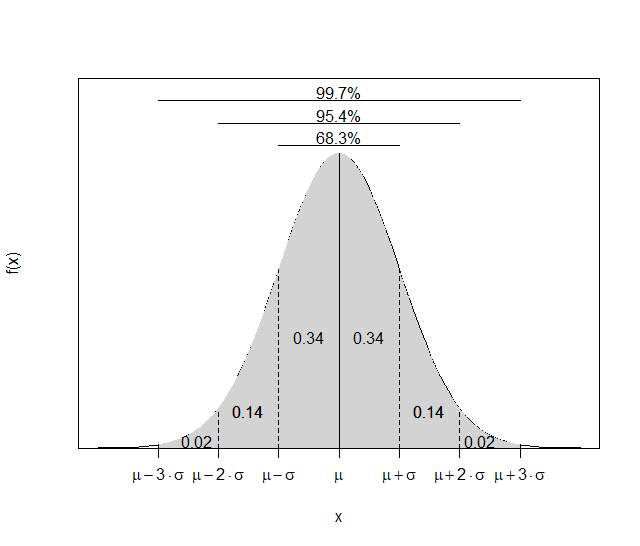
\includegraphics[scale=0.6]{figs/ICEmpirico.png}
			\end{figure}
			
		\end{block}
	\end{frame}
	
	\begin{frame}{Regra empírica para uma distribuição normal}
		\begin{block}{}
			\justifying
			Define-se \textbf{valores usuais} aqueles que são típicos e não muito extremos. Como sabemos que em uma distribuição (aproximadamente) normal, aproximadamente 95\% dos dados encontram-se a 2 desvios-padrões acima e
			abaixo da média, temos que
			\begin{align*}
				4\sigma &= (\max - \min) \\
				\sigma &= \frac{(\max - \min)}{4}
			\end{align*}
			pode ser utilizado como uma estimativa para $\sigma$.  
		\end{block}
	\end{frame}
	
	\begin{frame}{}
		\begin{block}{Exemplo}
			\justifying
			Um professor deseja estimar o salário médio de professores do Ensino Médio de uma cidade. Quantos professores devem ser selecionados para termos 90\% de confiança que a média amostral esteja a menos de R\$30,00 da média populacional? Sabe-se apenas que os
			salários variam entre R\$800,00 e R\$1.200,00. Use
			$$
			n = \left[ \frac{z_{\gamma/2} \cdot \sigma}{e} \right]^2
			$$  
			\nocite{Apostila}
			%\begin{verbatim}
			%zcrit <- qnorm(0.95)
			%erro <- 30
			%sigma <- (1200 - 800)/4
			%((zcrit * sigma)/erro)^2    
			%\end{verbatim}
		\end{block}
		\nocite{Morettin09, Apostila, eric, montgomery2016, meyer1982probabilidade, Bastos2025}
	\end{frame}
	
	\begin{frame}[allowframebreaks]
		\frametitle{\bf Referências}
		\printbibliography
	\end{frame}
	
	
\end{document}
